\chapter{Evaluation}
% Examiners expect to find in your dissertation a section addressing such questions as:

% \begin{itemize}
%    \item Were the requirements correctly identified?
%    \item Were the design decisions correct?
%    \item Could a more suitable set of tools have been chosen?
%    \item How well did the software meet the needs of those who were expecting to use it?
%    \item How well were any other project aims achieved?
%    \item If you were starting again, what would you do differently?
% \end{itemize}

% Other questions can be addressed as appropriate for a project.

% Such material is regarded as an important part of the dissertation; it should demonstrate that you are capable not only of carrying out a piece of work but also of thinking critically about how you did it and how you might have done it better. This is seen as an important part of an honours degree.

% There will be good things and room for improvement with any project. As you write this section, identify and discuss the parts of the work that went well and also consider ways in which the work could be improved.

% In the latter stages of the module, we will discuss the evaluation. That will probably be around week 9, although that differs each year.
The major requirements for this project were an IntelliJ Platform Plugin, back-end server, post-processor, front-end application, and a database. Each of these components were developed up to the point where they operate as intended. The settings GUI for the plugin was not implemented due to the using the continuous server architecture. Code generation, and code auto-completion of the source code detection types were not implemented due to the complexity of the identification process.

The primary design decision between using a continuous or non-continuous server architecture was a huge decision during this project. It impacted the method in which students would interact with the plugin and submit their tracked data. This in turn affected the back-end server internals. This decision was required before fully developing the server. If the continuous design was used then it would have most definitely increased the workload. Testing the direct connection between the plugin and server would be significantly more difficult than being able to individually test each component.

Using MongoDB was a very clear and strong design decision. If a RDBMS was to be used then the tracked data would need to be completely different from its current form. The use of Python has a clear advantage for using MongoDB. The simplicity of using dictionaries lead to simple interactions with the database.

If the project was to be written from scratch again, it would be interesting to have a greater focus on the post-processor. Concentrating more on the identification of possible cases of plagiarism would provide a much better result. It would be better due to the simplicity of the current identification algorithm being used. Integrating complex algorithms in the post-processor would allow for a more concrete result for each submission.

IntelliJ IDEA offers many ways to interact with the editor. Many were explored during the project including typing, copy and pasting, auto-completion, automatic code generation, and refactoring. Other methods that were not explored were using IdeaVim, and applying Git operations. IdeaVim emulates Vim in the editor. How would the use of this affect the detection methods? Would yank and paste still register as copy and paste? Using Git to stash changes, change branches, or even simply pulling from upstream can all modify files. Would these changes be tracked? If so, would this result in conflicts in the XML file? The XML file would need to be staged in each branch and commit before changing branch. Both IdeaVim, and Git could have been investigated.

\autoref{fig:velocity-chart} shows the velocity for each sprint. The average sprint velocity was 11. \autoref{fig:burndown-chart} shows the burndown for all iterations. Both of these charts show that development started well, slowed in the middle, and gained speed again towards the end. Using the scrum methodology proved successful for developing this project. It allowed, at maximum, a week to be wasted. If a waterfall approach was to be used, a lot more time could have been wasted if problems arose.

\begin{figure}[H]
  \centering
  \fbox{
    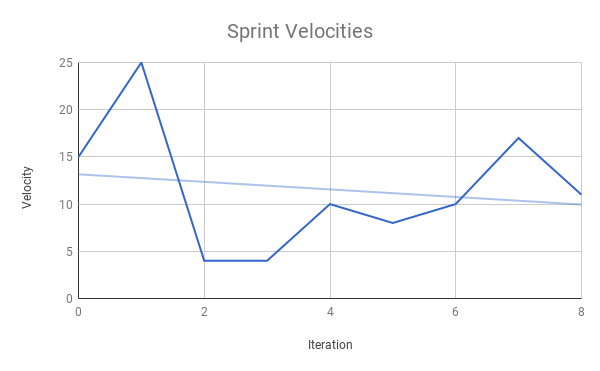
\includegraphics[height=\textheight,
    keepaspectratio=true,
    width=\textwidth,
    ]{figures/velocity-chart.png}
  }
  \caption[Velocity chart]{Velocity for each iteration}
  \label{fig:velocity-chart}
\end{figure}

\begin{figure}[H]
  \centering
  \fbox{
    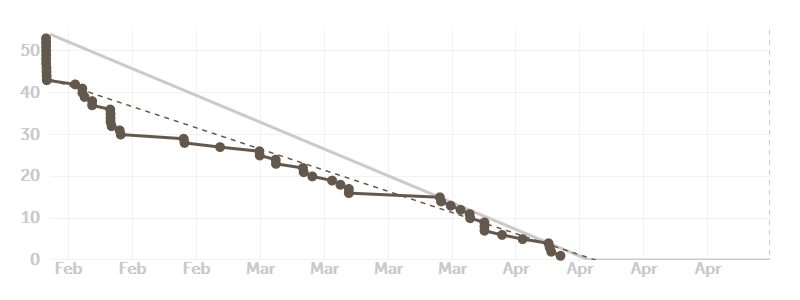
\includegraphics[height=\textheight,
    keepaspectratio=true,
    width=\textwidth,
    ]{figures/burndown-chart.png}
  }
  \caption[Burndown chart]{Burndown chart for all iterations}
  \label{fig:burndown-chart}
\end{figure}
